\section{Evaluation}
\label{sec:results}

In this section, we evaluate the performance of Matrix through
simulations. In Section \ref{subsec:sim} we describe the simulations
setup and used parameters. In Section \ref{subsec:res} we evaluate
the number of beacons transmitted, the usage of routing tables and
memory footprint, the downward routing success and response rate success and compare Matrix
with three state-of-the-art protocols: RPL~\cite{rfc6550}, CTP~\cite{Fonseca:2009} and
XCTP~\cite{xctp}. 

\subsection{Simulation setup}\label{subsec:sim}

Matrix was implemented as a subroutine of CTP in TinyOS \cite{tinyos}
and the experiments were run using the TOSSIM simulator \cite{tossim}. We
compare Matrix with and without the local broadcast mechanism, to which we refer
as MHCL. 

RPL was implemented in Contiki \cite{Dunkels:2004} and was
simulated on Cooja~\cite{Eriksson:2009}. Table \ref{tab:conf} lists the default
simulation parameters used for each protocol, in a non-faulty scenario. We use the $LinkLayerModel$ tool from TinyOS to generate the topology and connectivity model.

We simulated a range of faulty scenarios, based on experimental data collected
from TelosB sensor motes, deployed in an outdoor
environment \cite{Baccour:2012}. In each scenario, after every 60 seconds of
simulation, each node shutdowns its radio with probability $\sigma$ and keeps
the radio off for a time interval uniformly distributed in
$[\varepsilon - 5, \varepsilon + 5]$ seconds (see Table~\ref{tab:scn}).
The first scenario ($Scn1$) represents a network without node failures. The
remaining scenarios represent a combination of values of $\sigma$ and
$\varepsilon$. Note that these are all node-failure scenarios, which are
significantly harsher than models that simulate link or per-packet
failures only.

On top of the network layer, we ran two different applications: top-down and any-to-any. In the top-down application, each node sends 10 messages to the root and the root replies with an ack. In the any-to-any application, each node chooses randomly 10 destination addresses and sends one message to each of those addresses. Nodes start sending application messages 90 seconds after the simulation has started. The entire simulation takes 20 minutes. Each simulation was run 10 times. In each plot, the curve or bars represent the average, and the error bars the confidence interval of 95\%. For each protocol, only results relevant to each plot were included: e.g., CTP does not have a routing table nor performs top-down routing, and MHCL differs from Matrix only in faulty scenarios, otherwise it performs equally and therefore was omitted.

\begin{table}[!ht]
\centering
\caption{Simulation parameters}
\label{tab:conf}
\begin{tabular}{@{}lc@{}}
\toprule
\multicolumn{1}{l}{\textbf{Parameter}} & \textbf{Value} \\ \midrule
Base Station                           & 1 center       \\
Number of Nodes                        & 100            \\
Radio Range ($m$)                      & 100            \\
Density ($nodes/m^{2}$)                & 10             \\
Number of experiments                  & 10             \\
Path Loss Exponent                     & 4.7            \\
Power decay (dB)                       & 55.4           \\
Shadowing Std Dev (dB)                 & 3.2            \\
Simulation duration                    & 20 min            \\
Application messages                   & 10 per node \\
Max. Routing table size                & 20 entries \\
\bottomrule
\end{tabular}
\end{table}



\begin{table}[!ht]
\centering
\caption{Faulty network scenarios}
\label{tab:scn}
\begin{tabular}{|c|c|c|c|}
\hline
\textbf{$\sigma$$\setminus$$\varepsilon$} & \textbf{10 s} & \textbf{20 s} & \textbf{40 s}\\ \hline
\textbf{1\%}     & Scenario 2            & Scenario 3        & Scenario 4              \\ \hline
\textbf{5\%}     & Scenario 5            & Scenario 6        & Scenario 7             \\ \hline
\textbf{10\%}    & Scenario 8            & Scenario 9        & Scenario 10              \\ \hline
\end{tabular}
\end{table}


\subsection{Results}\label{subsec:res}

Firstly, we turn our attention to memory efficiency of each protocol. To evaluate the usage of routing tables, we compare the number of entries used by each protocol. Each node was allocated a routing table of maximum size equal to 20 entries.
In Figure \ref{fig:table-usage}, we show the CDFs (cumulative distribution
functions) of the percentage of routing table usage among nodes\footnote{We
measured the routing table usage of each node in one-minute intervals, then
took the average over 20 minutes.}, and compare Matrix, RPL, XCTP, and MHCL.

In this plot, Matrix was simulated in the faulty scenario \#10 (Table \ref{tab:scn}).
Note that $>35\%$ of nodes are leaves, i.e., do not have any descendants in the collection tree topology, and therefore use zero routing table entries.

As we can see, RPL is the only protocol that uses 100\% of table
entries for some nodes ($\geq30\%$ of nodes have their tables full).
This is due to the fact that RPL, in the storing mode, pro-actively
maintains an entry in the routing table of every node on the path
from the root to each destination, which quickly fills the available
memory and forces packets to be dropped.

XCTP reactively stores reverse routes only when required. Therefore, the number of routing
entries used by XCTP depends on the number of data flows going through each node. Since the simulated flows were widely spaced during the simulation time, the XCTP was able to perform efficiently.

The difference between MHCL and Matrix is small: MHCL
stores only the IPtree structure, whereas Matrix stores IPtree and
RCtree data; the latter is kept only temporarily during parent
changes in the collection tree, so its average memory usage is low.

\begin{figure}[h]
    \centering
    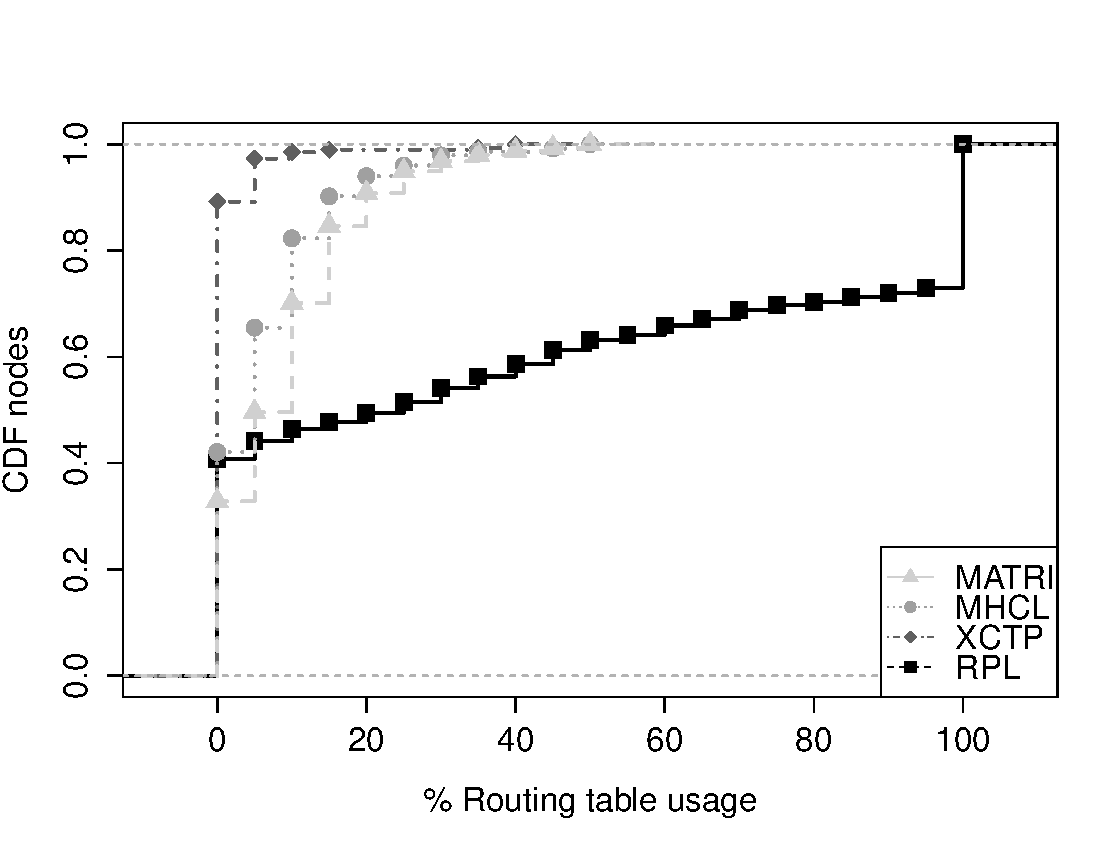
\includegraphics[width=1\linewidth]{Images/tableusagex.pdf}
    \caption{Routing table usage CDF. (Maximum table size = 20)}
    \label{fig:table-usage}
\end{figure}

Figure \ref{fig:beacons} illustrates the amount of control traffic
in our experiments (the total number of beacons sent during the entire simulation). Matrix sends fewer control packet than RPL, because it only sends additional beacons during network initialization and in case of collection tree topology updates, whereas RPL has a communication intensive maintenance of downward routes during the entire execution time. Since XCTP is a reactive protocol, it does not send additional control packets, when compared to CTP.

\begin{figure}[h]
    \centering
    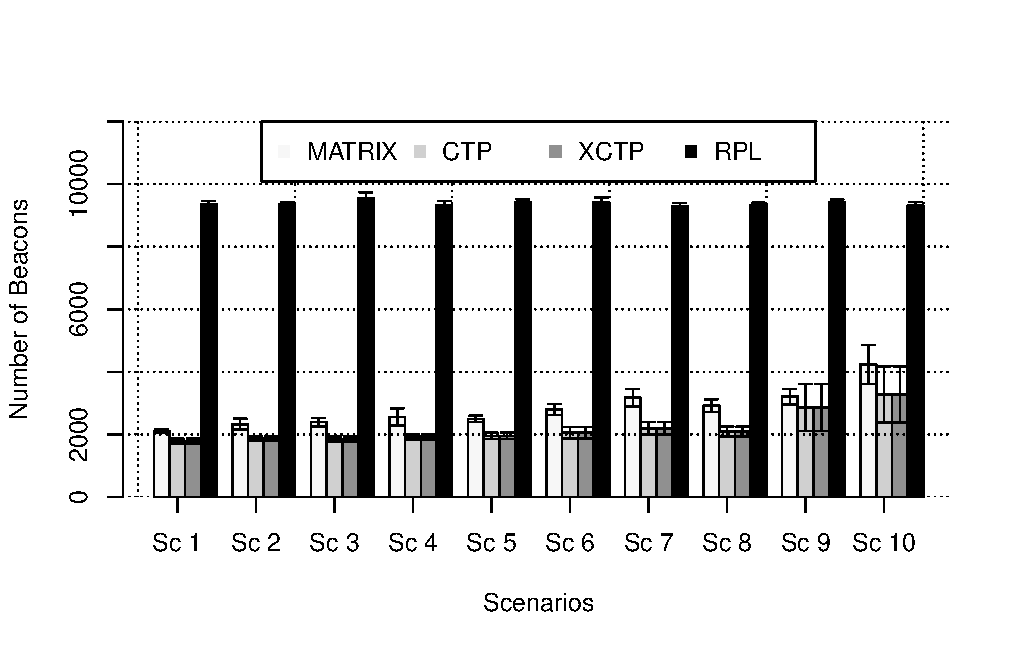
\includegraphics[width=1\linewidth]{Images/beacons.pdf}
    \caption{Number of control packets.}
    \label{fig:beacons}
\end{figure}

Figure~\ref{fig:footprint} compares RAM and ROM footprints in the protocol stack of CTP, RPL, XCTP, and Matrix. We can see that Matrix adds only a little more than 7KB of code to CTP, allowing this protocol to perform any-to-any communication with high scalability. When compared with RPL, the execution code of Matrix requires less RAM. Compared to XCTP, Matrix uses almost the same amount of RAM.

\begin{figure}[h]
    \centering
    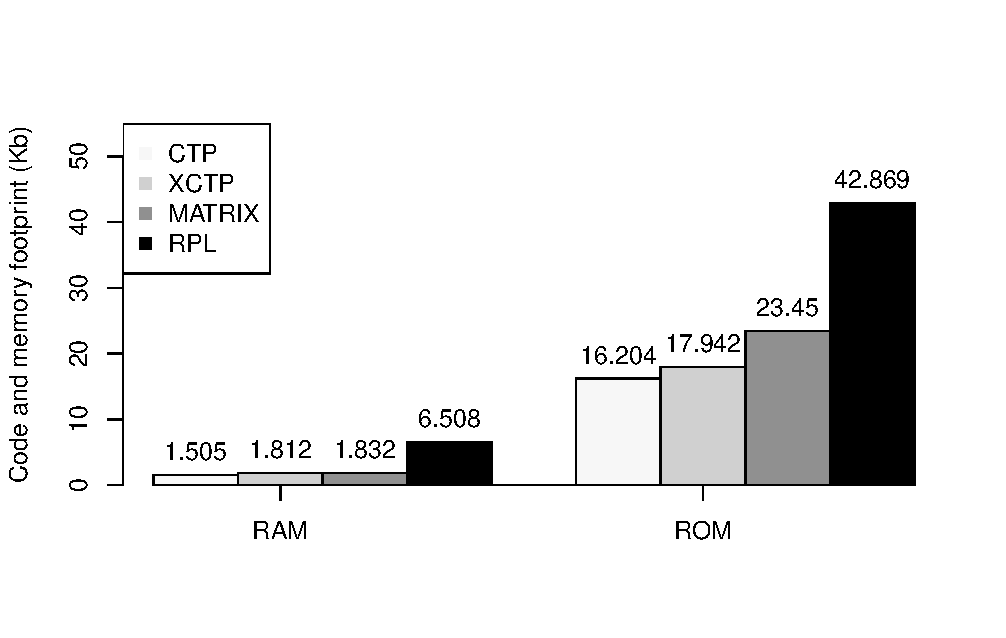
\includegraphics[width=1\linewidth]{Images/footprint.pdf}
    \caption{Code and memory footprint in bytes.}
    \label{fig:footprint}
\end{figure}

In Figure~\ref{fig:txdwn} we compare top-down routing success rate. We measured the total
number of application (ack) messages sent downwards and successfully received by
the destination.\footnote{We do not plot the success rate of bottom-up traffic,
since it is done by the underlying collection protocol, without any
intervention from Matrix.} In the plot, ``inevitable losses'' refers to the
number of messages that were lost due to a failure of the destination node, in which case, there were no valid path to the destination and the packet loss was inevitable.
The remaining messages were lost due to wireless collisions and node failures on
the packet's path. 

We can see that, when a valid path exists to the destination, the top-down success rate of Matrix varies between 95\% and 99\%. In the harshest faulty scenario 10, without the local broadcast mechanism, MHCL delivers 85\% of top-down messages. With the local broadcast activated, the success rate increases to 95\%, i.e., roughly 2/3 of otherwise lost messages succeed in reaching the final destination.
Note that external factors may be causing RPL's low success rate. Since RPL was the only protocol implemented on Contiki and evaluated in Cooja, native protocols from this OS can interfere on the results. In \cite{Bezunartea:2016}, the authors show how different radio duty cycling mechanisms affect the performance of a RPL network. However, RPL delivered less than $20\%$ of messages in all simulated scenarios, which occurs due to lack of memory to store all the top-down routes.  Since XCTP is a reactive protocol, it adapts best to failures and dynamics, because downward routes are updated when a message travels upwards. In this way, the top-down success rate of XCTP is higher even in the presence of failures.

\begin{figure}[h]
    \centering
    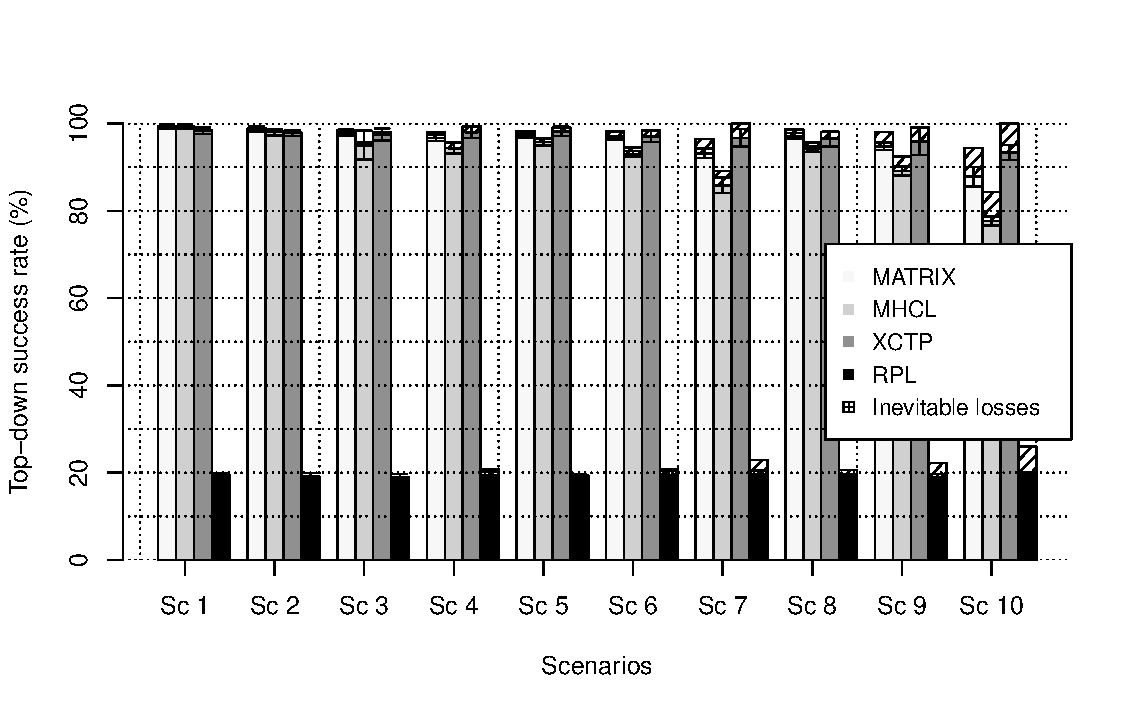
\includegraphics[width=1\linewidth]{Images/txrouting.pdf}
    \caption{Top-down routing success rate.}
    \label{fig:txdwn}
\end{figure}

In Figure~\ref{fig:txany} we compare the any-to-any success rate. We measured the total number of messages sent by a node that was successfully received by the destination. In this application, each node chooses randomly a destination address and sends a message to this node. We can see that, as expected, there is no big difference between any-to-any and top-down traffic patterns. Matrix performs any-to-any routing with 90\% to 100\% success rate, when a valid path exists to the destination. The success rate of RPL remains low, due to lack of memory to store all the routing information needed. 

\begin{figure}[h]
    \centering
    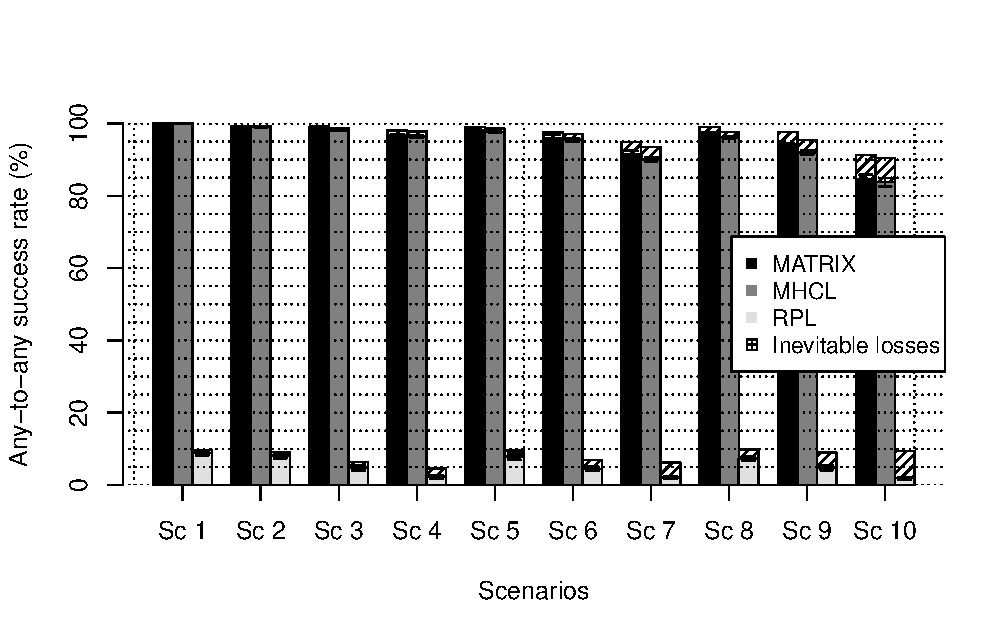
\includegraphics[width=1\linewidth]{Images/anytoany.pdf}
    \caption{Any-to-any routing success rate.}
    \label{fig:txany}
\end{figure}


Finally, in Figure~\ref{fig:txrsp} we compare the response rate of Matrix and XCTP. We calculate the response rate by dividing the number of acknowledgements sent by the root by the number of messages received by the root. We vary the response delay, that is, upon receiving a message, the root will reply with an acknowledgment after $x$ milliseconds, $x \in\ \{100,200,225,250,275,300,325,350,375,400,800\}$. We can see that the performance of XCTP is highly dependent on the number of data flows. By increasing the application response delay, the number of simultaneous flows increases and the response success rate decreases, because nodes can not store all the information needed. Matrix, on the other hand, does not depend on the number of flows, and the routing table usage is bounded by the number of children of each node.

\begin{figure}[h]
    \centering
    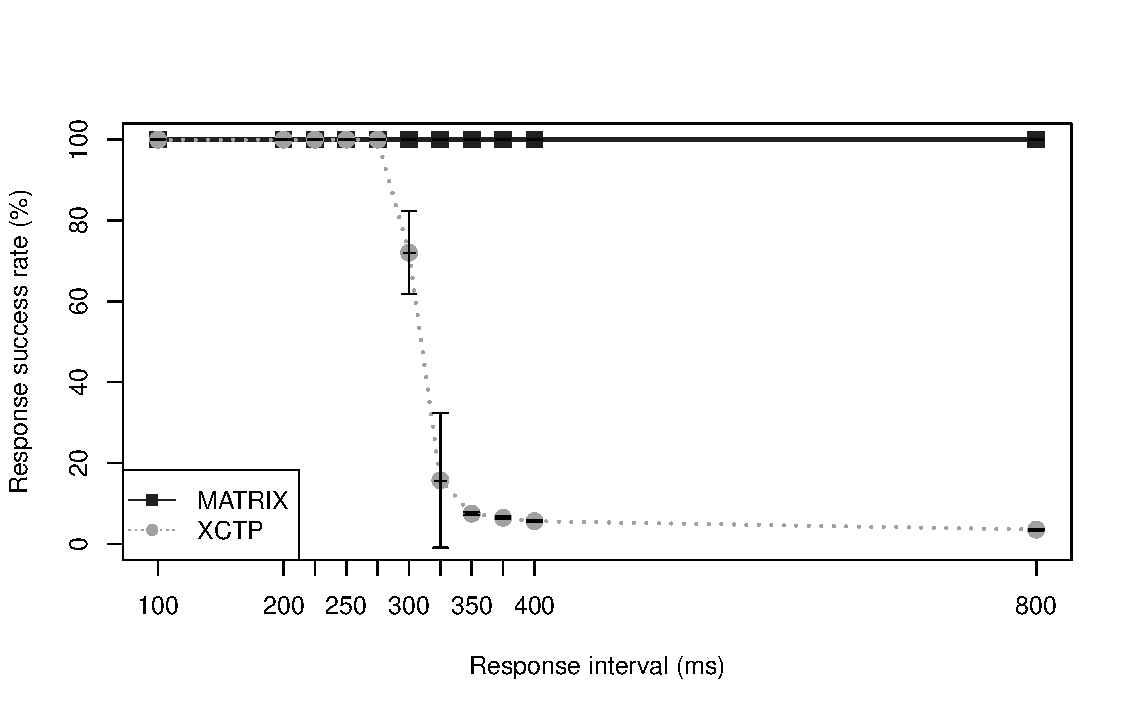
\includegraphics[width=1\linewidth]{Images/rsprate.pdf}
    \caption{Response success rate.}
    \label{fig:txrsp}
\end{figure}